\subsection{Data processing}
In listing \ref{lst:sql-roads} (Appendix), the query that is used to extract
all roads in an area is listed. This query is used inside an \url{f-string}
in \url{Python}, to be able to loop over the different areas and extract
the roads from it. Note that a buffer of a few meters around the neighborhood
is used for the filtering, since otherwise this results in edge cases,
where a road is ever so slightly more to the outside of the area than the boundary,
and it would get left out. \url{ST_Intersects} is used to extract all roads
that are at least partly inside or on the boundary. A similar query is used 
to extract the nodes, but this is easier since for a building which is only
defined by a single node, it is not needed to define a new geometry object.

One of the predictors of the TSP path length, is the area of the neighborhood
the locations are drawn from. The OSM data provides the area of the polygons,
but this value can not be used to predict TSP path length effectively.
This value is a heavy overestimation of the correct value for $A$.
In many cases, there are parts of the neighborhood that do not contain
any buildings, for instance when there is a park in the neighborhood. To
account for this, the value for $A$ that is used, is the area of the convex
hull around all buildings, which is calculated using the \url{shapely}
module in \url{Python}. As an example visualization, figure \ref{fig:binnenstad_quarter} displays
how the quarter for the inner city of Groningen is defined in OpenStreetMap. Using the area of this
entire quarter would be an overestimation. A significant portion of this area is the canal and outer
road around the inner city. There are many examples of quarters where this overestimation is even
more significant than this.
\begin{figure}[H]
  \caption{The OpenStreetMap quarter for the inner city of Groningen (Binnenstad). \citep{openstreetmap}}
  \label{fig:binnenstad_quarter}
  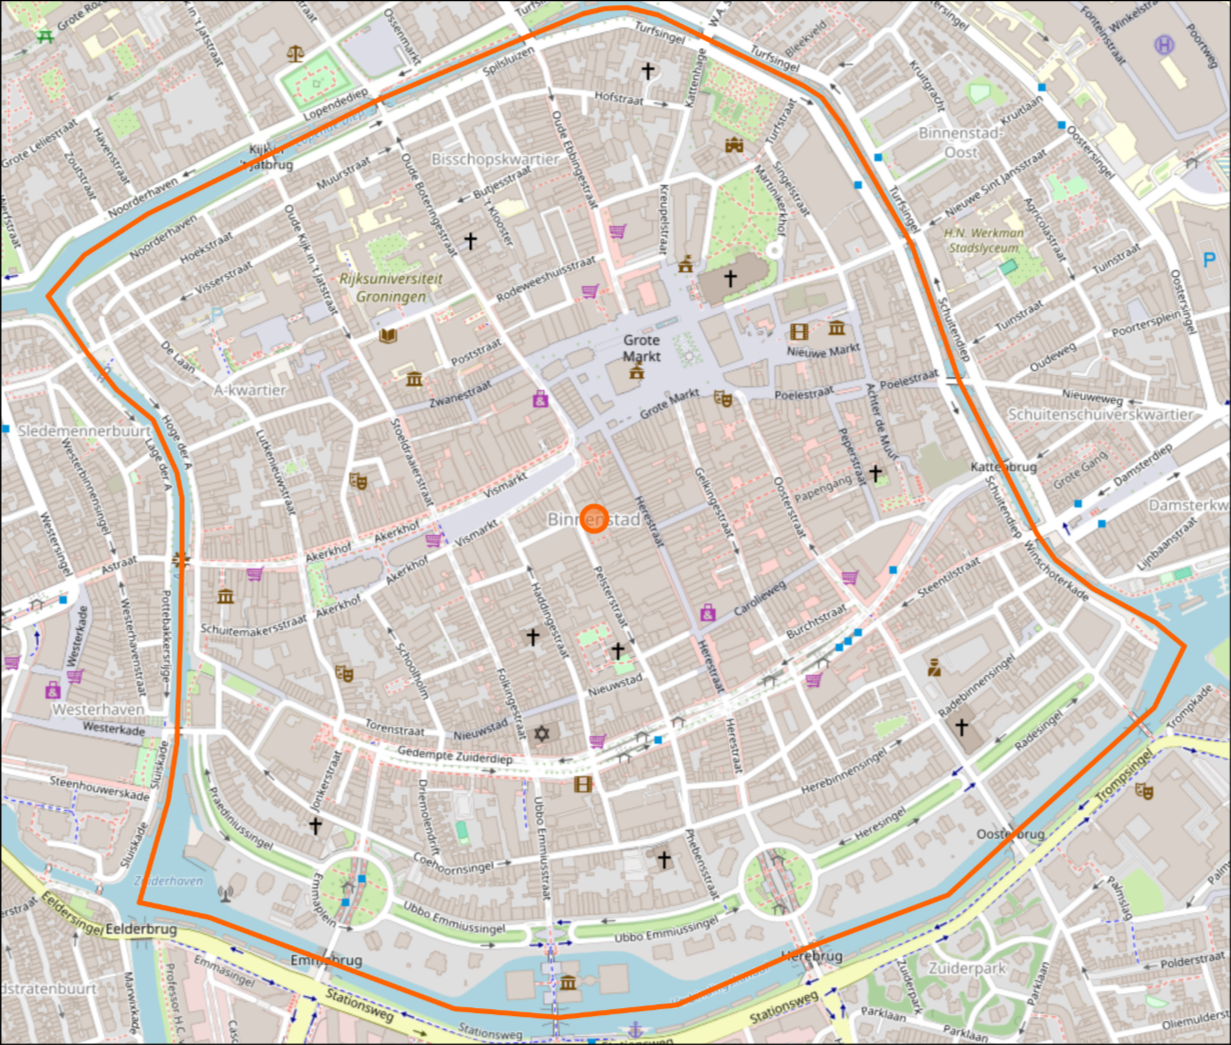
\includegraphics[width=\textwidth]{Pictures/Binnenstad_quarter.png}
\end{figure}
Using the geographic information of the roads and buildings, a graph
is constructed, using the \url{igraph} module in \url{Python}. This graph
connects all buildings to each other over the road network. First, using the information about the 
roads and buildings the sets of nodes and edges need to be defined. An edge is a line that connects
two edges to each other. Extracting the edges that connect the road network is straightforward,
since all roads already have an ordered list of nodes defined. The subsequent nodes simply need to
be stored as pairs, and all edges are defined.

When the road network is defined as a set of nodes and edges, the next step is to connect the buildings
to the road network. This needs to be done manually, since no data is stored in OpenStreetMap 
about to which road the buildings belong. This algorithm needs to be very efficient, since many 
buildings are added in each area. An R-tree can be used to accomplish this efficiency.
An R-tree is a dynamic index structure that is able to retrieve data items quickly according to 
their spatial locations \citep{guttman1984r}. Listing \ref{lst:python-edges} displays the algorithm
used to make the edges that connect the buildings to the road network. For each building node,
the closest point on the closest road is found, using the shapely implementation of the R-tree,
\url{STRtree}. Then, if this point is not an already existing node, a new virtual node is added,
which splits this existing edge in two parts. The road is reconnected with the new node in between.
Finally, the building is connected to this new node.

In order to find the shortest path in terms of real distance, and to calculate the length of the 
TSP path, a 'weight' needs to be added. This weight represents the length of this edge in meters.
The equirectangular approximation is used to calculate these weights. This approximation is very
efficient, but only works when the points the distance is calculated between is small enough such
that the rounding of the earth does not have a significant effect on the true distance.
The nodes are all close enough together, so the effect of the 
rounding of earth's surface is negligible. Let $A$ and $B$ be two nodes,
and $(x_A,y_A)$, $(x_B),y_B)$ be their coordinates, in \url{radians}. Let $R=6,371,000$ meters, 
Earth's radius. Then the distance between these nodes (the weight of the edge connecting them),
using the equirectangular approximation is:
\begin{align}
  \label{eq:equirectangluar_approx}
  d(A,B)	&=R\sqrt{x^2+y^2},\\
  \text{where }x&=(x_B-x_A)\cos{\frac{y_A+y_B}{2}},\\
  \text{and }y	&=y_B-y_A.
\end{align}

Using the \url{folium} module in \url{Python}, such a graph can be projected back onto the world map.
One of such visualizations is provided in figure \ref{fig:overtoomse_sluis}. All maps like this one,
for the areas in this analysis can be viewed and interacted with via this 
\href{https://koenstevens.nl/wp-content/uploads/maps/}{\url{webpage}}.
\begin{figure}[H]
  \caption{Visualization of the graph, for the Overtoomse Sluis quarter in Amsterdam.}
  \label{fig:overtoomse_sluis}
  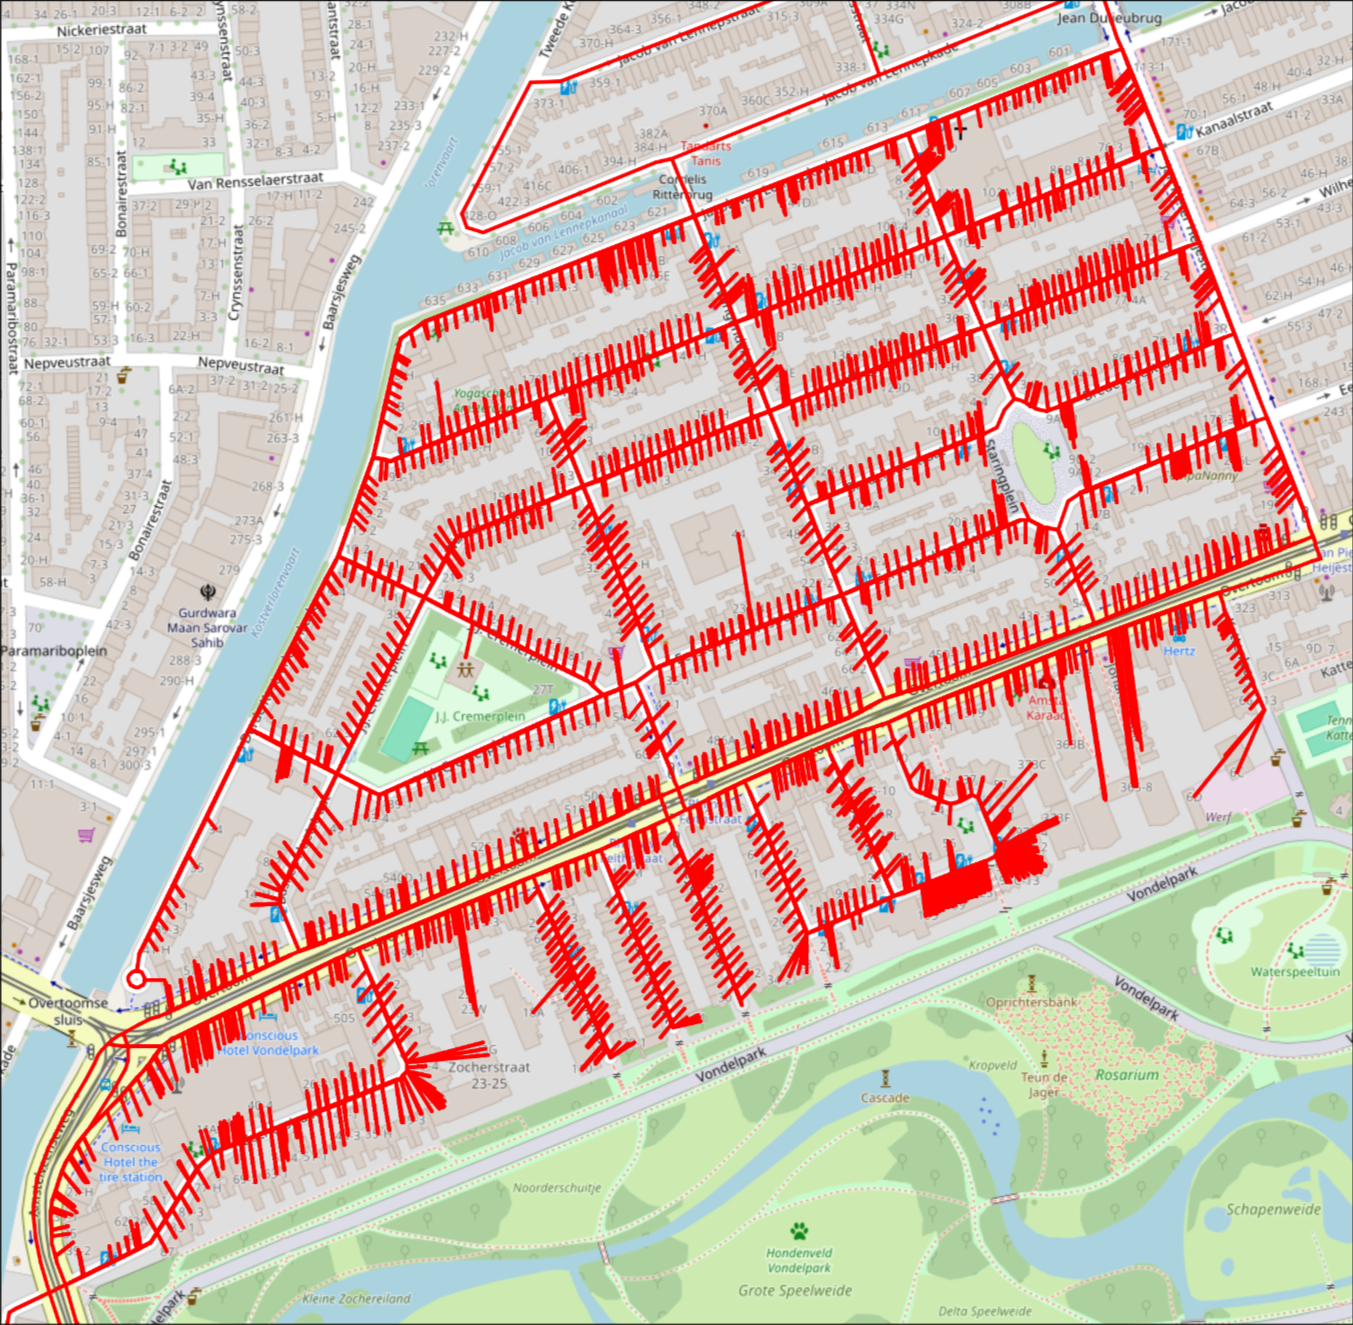
\includegraphics[width=\textwidth]{Pictures/Overtoomse_Sluis_roads.png}
\end{figure}
